\subsection{Komponen \textit{Rule Manager}}
Komponen \textbf{\textit{Rule Manager}} berfungsi untuk melakukan parsing terhadap file \textit{rule} yang telah diisi oleh pengguna serta menjadi aggregator untuk melakukan pengecekan \textit{rule} yang berlangsung serta memberi informasi data prediksi kapan saja yang dibutuhkan untuk melakukan pengecekan. Parsing komponen ini menggunakan format csv dan kondisi diekspresikan dengan sintaks python. Komponen akan mengonstruksi objek \textbf{\textit{Rule}} yang akan digunakan oleh komponen \textbf{\textit{Flexible Control}}. Agar terbayang, contoh dari \textit{file rule} dapat dilihat pada gambar \ref{fig:rule-example}. Spesifikasi dari kedua kelas tersebut dapat dilihat pada gambar \ref{fig:rule-spek}.

\begin{figure}[h]
    \centering
    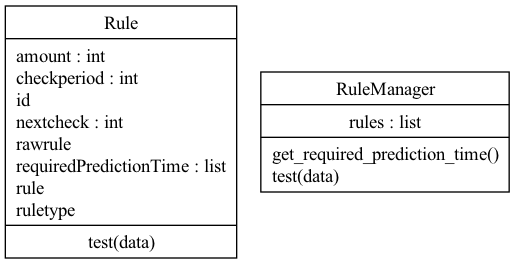
\includegraphics[width=0.8\textwidth]{chapter-4/rule.png}
    \caption{Spesifikasi Kelas Penyusun Komponen \textit{Rule Manager}}
    \label{fig:rule-spek}
\end{figure}

\begin{figure}[h]
    \centering
    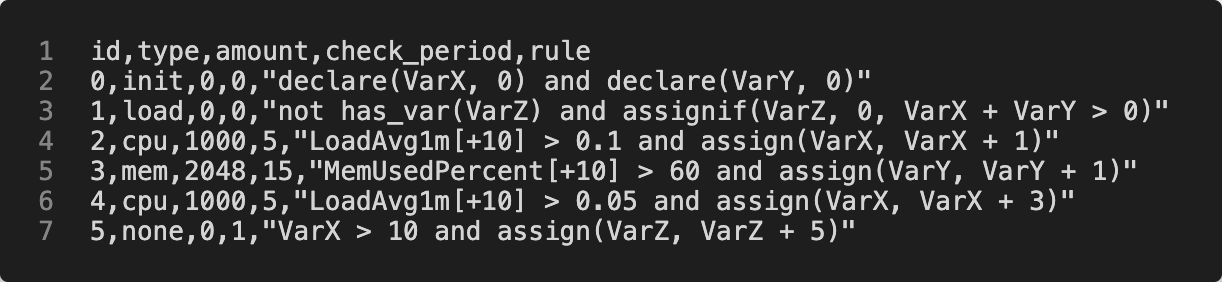
\includegraphics[width=0.75\textwidth]{chapter-4/cth-rule.png}
    \caption{Contoh \textit{File Rule}}
    \label{fig:rule-example}
\end{figure}

Sebuah \textit{rule} memiliki fungsi sebagai berikut.
\begin{enumerate}
    \item Memiliki sebuah kondisi yang akan dievaluasi dengan data prediksi pada waktu prediksi yang diinginkan. Contoh: kondisi \textit{throughput} untuk operasi X untuk 1 menit kedepan dan 5 menit kedepan lebih dari 1s, maka tingkatkan prosesor sebanyak 500m.
    \item Memiliki jumlah serta target kategori untuk diubah, dalam kasus ini pilihannya memori atau prosesor.
    \item Satuan untuk perubahan memori adalah dalam \textit{Mebibyte} atau MiB. Sedangkan untuk prosesor dalam satuan mili atau m.
    \item Sebuah \textit{rule} memiliki periode pengecekan sehingga tidak akan dicek secara terus menerus yang menyebabkan perubahan alokasi sumber daya terlalu cepat. Periode pengecekan dibuat dalam satuan sekon.
\end{enumerate}

Seperti yang bisa dilihat pada contoh gambar \ref{fig:rule-example}, untuk membuat sebuah \textit{rule}, terdapat 5 buah \textit{field} yang harus diisi. \textit{Field} tersebut adalah sebagai berikut.
\begin{enumerate}
    \item \textbf{ID}

        \textit{Field} ini dibebaskan kepada pengguna dan bertipe \textit{string} dan akan digunakan untuk mengidentifikasi \textit{rule} yang dibuat terutama jika terjadi error.
    \item \textbf{\textit{Type}}
    
        \textit{Field} ini bertipe \textit{string} dan akan digunakan untuk mengidentifikasi tipe eksekusi \textit{rule}. Berikut adalah pilihan yang dapat digunakan.
        \begin{enumerate}
            \item \textbf{\textit{Init}}
            
                \textit{Rule} akan otomatis berjalan diawal saat inisiasi (saat pertama kali dijalankan ataupun setelah di-\textit{reset}). Kategori pilihan ini digunakan untuk mendeklarasikan variabel \textit{user-defined} yang bisa digunakan untuk kondisi kompleks atau \textit{rule} yang saling berkaitan.

            \item \textbf{\textit{Load}}
            
                Berbeda dengan inisiasi, \textit{rule} ini akan berjalan ketika sistem dinyalakan dalam kondisi melanjutkan atau sesudah \textit{restart}. Kategori pilihan ini digunakan untuk mendeklarasikan variabel \textit{user-defined} yang mungkin ditambahkan saat \textit{restart}. Pada contoh gambar \ref{fig:rule-example}, dideklarasikan variabel $VarZ$ apabila belum terdefinisi dan $VarX+VarY > 0$.

            \item \textbf{\textit{None}}
            
                \textit{Rule} ini akan berjalan secara periodik namun tidak mengubah alokasi sumber daya apapun. Dapat digunakan untuk melakukan \textit{update} terhadap variabel \textit{user-defined}.

            \item \textbf{\textit{CPU}}

                Seperti namanya, digunakan untuk mengubah alokasi prosesor jika kondisi terpenuhi.
            \item \textbf{\textit{Mem}}
            
            Seperti namanya, digunakan untuk mengubah alokasi memori jika kondisi terpenuhi.
        \end{enumerate}

    \item \textbf{\textit{Amount}}
    
        \textit{Field} ini hanya berguna apabila tipe \textit{rule} adalah \textbf{CPU} atau \textbf{Mem}. Seperti namanya, digunakan untuk mengatur jumlah perubahan. Untuk \textbf{CPU}, angka dalam satuan milli. Sedangkan, untuk \textbf{Mem}, angka dalam satuan \textit{Mebibyte} (MiB).
    
    \item \textbf{\textit{Check Period}}
        
        \textit{Field} ini digunakan untuk mengatur periode pengecekan dalam satuan sekon. Periode ini berfungsi sebagai \textit{cooldown} jika kondisi bernilai benar. Setiap \textit{rule} yang ada akan dicek secara global setiap sekon, namun jika sudah bernilai benar, akan memasuki periode tidak dicek sampai periode pengecekan selesai. Jika kondisi bernilai salah, maka akan dicek kembali pada detik berikutnya. Tidak berlaku untuk tipe \textbf{init} dan \textbf{load} karena dua tipe tersebut akan selalu dijalankan sekali pada saat inisiasi atau \textit{restart}.

    \item \textbf{\textit{Rule}}
        
        \textit{Field} ini berisikan kondisi yang akan dievaluasi. Kondisi ini harus berupa ekspresi boolean yang terdiri dari variabel \textit{user-defined}, variabel prediksi metrik sistem dan operator logika. Variabel \textit{user-defined} dapat berupa variabel yang dideklarasikan pada \textit{rule} dengan tipe \textbf{init} atau \textbf{load} atau variabel yang dideklarasikan pada \textit{rule} lainnya. Operator logika yang dapat digunakan adalah \textbf{and}, \textbf{or}, dan \textbf{not}. Untuk operator perbandingan yang dapat digunakan adalah \textbf{$==$}, \textbf{$!=$}, \textbf{$>$}, \textbf{$>=$}, \textbf{$<$}, dan \textbf{$<=$}. Untuk operator aritmatika yang dapat digunakan adalah \textbf{+}, \textbf{-}, \textbf{*}, \textbf{/}, dan \textbf{\%}.

        Terdapat batasan berupa tidak bisa meletakkan variabel prediksi metrik sistem pada \textit{rule} bertipe \textbf{init} dan \textbf{load}. Apabila ingin menggunakan variabel prediksi metrik sistem, maka harus menggunakan tipe \textbf{CPU} atau \textbf{Mem}.

        Untuk variabel \textit{user-defined}, batasan yang ada adalah penamaan variabel harus dilakukan layaknya \textit{script} pada umumnya, seperti tidak bisa dimulai dengan angka, namun bisa diakhiri oleh angka dan tidak boleh mengandung simbol selain garis bawah.

        Sedangkan, untuk variabel metrik sistem yang dapat digunakan adalah sebagai berikut.

        \begin{enumerate}
            \item \textbf{\textit{Write Load}}
            \item \textbf{\textit{Index}}\label{item:index}
            \item \textbf{\textit{Get}}
            \item \textbf{\textit{Query}}
            \item \textbf{\textit{Fetch}}
            \item \textbf{\textit{Scroll}}
            \item \textbf{\textit{Suggest}}
            \item \textbf{\textit{Bulk}}
            \item \textbf{\textit{Flush}}
            \item \textbf{\textit{Refresh}}\label{item:refresh}
            \item \textbf{\textit{CPUPercent}}\label{item:cpupercent}
            \item \textbf{\textit{LoadAvg1m}}\label{item:load-avg-1}
            \item \textbf{\textit{LoadAvg5m}}
            \item \textbf{\textit{LoadAvg15m}}\label{item:load-avg-15}
            \item \textbf{\textit{MemUsedPercent}}\label{item:mempercent}
        \end{enumerate}

        Untuk nomor \ref{item:index} sampai \ref{item:refresh} adalah \textit{throughput} operasi-operasi \textit{Elastic Search} dalam bentuk milisekon. Sedangkan, \ref{item:cpupercent} dan \ref{item:mempercent} adalah pemakaian CPU dan memori dalam bentuk bilangan bulat 1-100 yang merepresentasikan persen pemakaian. \textit{Load Average} adalah indikator beban sistem dalam 1, 5, dan 15 menit terakhir. Biasanya angka ini digunakan untuk menentukan turun naiknya beban prosesor sistem. Apabila menunjukkan kenaikan, maka dapat dipastikan bahwa sistem mulai digunakan. Sedangkan, apabila menunjukkan penurunan, maka sistem mulai tidak digunakan. Persamaan \ref{eq:load-average} akan digunakan untuk menjelaskan angka pada \textit{Load Average}. Pada persamaan tersebut, $U(t)$ adalah persen utilisasi di waktu $t$. Sebagai contoh, ketika $LoadAvg(t)$ bernilai $1.0$ dan $NumberOfCPU$ adalah $4$, maka dapat disimpulkan bahwa persentase utilisasi CPU adalah $25\%$ sehingga bisa disimpulkan sebagai sistem belum maksimal dimanfaatkan. Namun, variabel ini biasanya bercampur juga dengan utilisasi prosesor dari sistem, jaringan, file I/O dan network I/O berbeda dengan \textit{CPUPercent} yang murni menunjukkan utilisasi prosesor dari sistem untuk proses \textit{Elastic Search}.

        \begin{equation}
            \label{eq:load-average}
            U(t) = LoadAvg(t)/NumberOfCPU*100
        \end{equation}
\end{enumerate}